% !TeX root = f44_shortreport_schmitt_kleinbek.tex
\section{Measurements Log and Evaluation}
\subsubsection{First Part: Spectroscopy of the Zeeman effect}
In the first part of the experiment, the Zeeman effect was investigated using the red cadmium line, which ist formed at the transition from $^1\text{D}_2\rightarrow ~^1\text{P}_1$.\\

To this end, it should first be examined whether a hystheresis effect occurs with the magnets used.
For this purpose, three measurements were performed with a Hall probe each with increasing and decreasing field strength in the relevant range and the results for $B_\text{inc}$ and $B_\text{dec}$ were averaged.
In Figure \ref{fig:hystheresis} you see the results of this measurement.
\begin{figure}[ht]
\centering
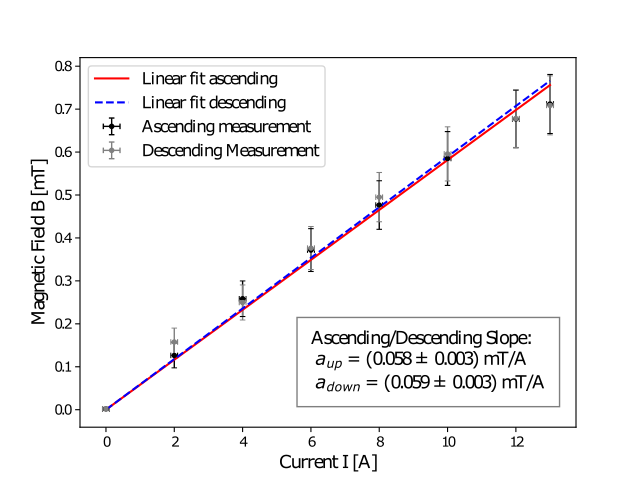
\includegraphics[scale=.55]{images//hystheresis.png}
\caption{Comparison of the magnetic field strength with increasing and decreasing current strength}
\label{fig:hystheresis}
\end{figure}
You can see that there is a small difference between the measurements, but the fit reveals that this difference is within the error, which is why in our case there is no significant effect.\\

Next, the Zeeman effect should be qualitatively investigated in longitudinal and transverse direction.
For this purpose, we used the structure shown in figure \ref{fig:structure}.
\begin{figure}[ht]
\centering
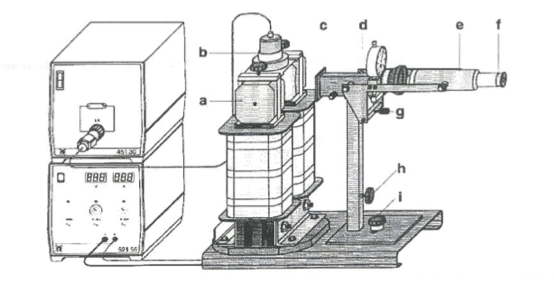
\includegraphics[scale=.9]{images//structure.png}
\caption{Experimental set-up: a) Pole pieces of the magnet, b) Cd lamp, c) Red light filter, d) Lummer-Gehrcke Plate, e) Telescope, f) Eyepiece, g) Height adjustment for the telescope, h) Locking screw for the telescope holder, i) Locking screw for the base plate. \cite{leaflets}}
\label{fig:structure}
\end{figure}
The most important element of this construction is the Lummer-Gehrcke plate with almost plane-parallel surfaces.
If light enters the plate trough a prism with an angle of incidence of $\beta$, it is reflected inside the plate.
After each reflection some light is refracted at the surface, which is focused with the help of a lens and brought to interference.\\
If the gait difference meets the conditions
\begin{align}
\Delta = 2d\sqrt{n^2-1} = k \lambda
\end{align}
constructive interference with the gear difference $\Delta=\Delta_1-\Delta_2$, the refractive index $n=n_2$ and $n_1\approx1$, the thickness of the plate $d$ and the interference order $k$ is obtained.
The reflection angle $\alpha$ within the plate is assumed to be approximately $90°$, resulting in near total reflection within the plate.\\
Our interference pattern of the Lummer-Gehrcke plate for a transversal image can be seen in Figure \ref{fig:interference}.
\begin{figure}[ht]
\centering
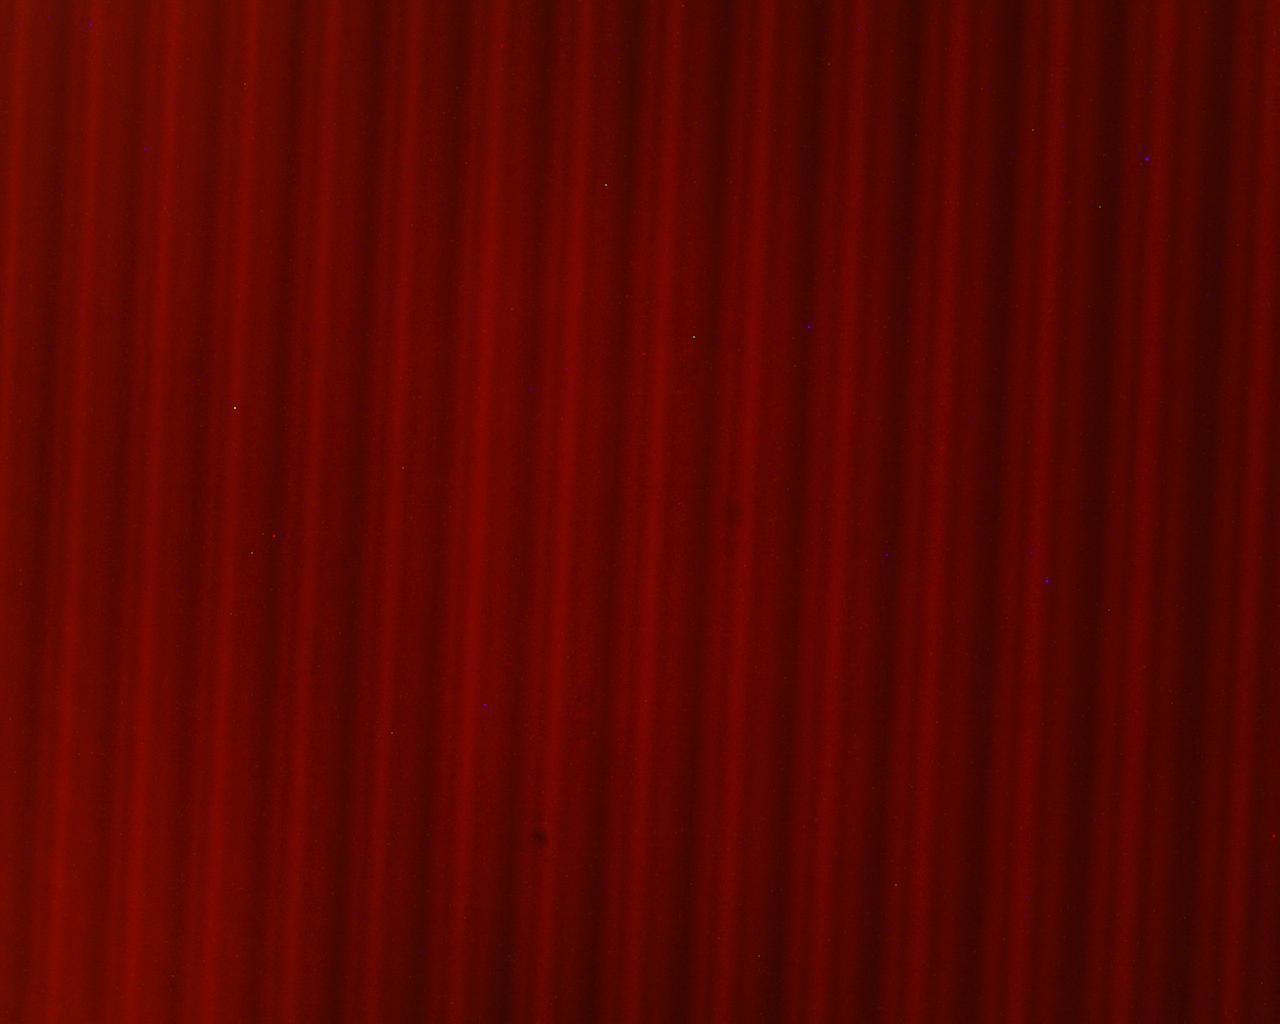
\includegraphics[scale=.15]{images//interference.jpg}
\caption{Zeeman effect in transverse direction at $I=13$A}
\label{fig:interference}
\end{figure}

\subsubsection{Second Part: Precision spectroscopy}